
\documentclass{article} % For LaTeX2e
\usepackage{iclr2026_conference,times}

\usepackage{hyperref}
\usepackage{url}
\usepackage{graphicx}
\usepackage{booktabs}
\usepackage{amsmath}
\usepackage{amssymb}
\usepackage{float}

% Spacing compaction
\setlength{\textfloatsep}{6pt plus 2pt minus 2pt}
\setlength{\floatsep}{6pt plus 2pt minus 2pt}
\setlength{\intextsep}{6pt plus 2pt minus 2pt}
\setlength{\dbltextfloatsep}{6pt plus 2pt minus 2pt}
\setlength{\dblfloatsep}{6pt plus 2pt minus 2pt}
\setlength{\abovecaptionskip}{2pt}
\setlength{\belowcaptionskip}{0pt}
\setlength{\abovedisplayskip}{5pt plus 2pt minus 2pt}
\setlength{\belowdisplayskip}{5pt plus 2pt minus 2pt}

% Bibliography compaction (natbib defines \bibsep; guard in case the style changes)
\makeatletter
\@ifundefined{bibsep}{\newlength{\bibsep}}{}
\makeatother
\setlength{\bibsep}{0pt plus 0.3ex}
\setlength{\parskip}{0pt plus 1pt}
\raggedbottom

\title{Lite MTP: Minimalist Multi-Token Prediction for Edge Architectures}

% Authors must not appear in the submitted version. They should be hidden
% as long as the \iclrfinalcopy macro remains commented out below.
% Non-anonymous submissions will be rejected without review.

\author{Anonymous}

\newcommand{\fix}{\marginpar{FIX}}
\newcommand{\new}{\marginpar{NEW}}

%\iclrfinalcopy % Uncomment for camera-ready version, but NOT for submission.
\begin{document}


\maketitle

\begin{abstract}
Speculative Decoding (SD) exploits the memory-bound nature of Large Language Model (LLM) generation to hide the compute cost of drafting and running multiple tokens through a single model forward pass \citep{leviathan2023fast, chen2023accelerating}. Modern SD techniques such as Medusa and Eagle are designed to maximize operational intensities, so they are highly effective for GPUs, but not Edge devices\citep{cai2024medusa, li2024eagle}. Additionally, they increase the parameter count with their draft-heads, negating the benefits of the small architecture. In this work, we evaluate Medusa's independent head and Eagle's sequential feature architectures on Gemma 3 270M \citep{google2024gemma}, comparing performance between Nvidia A100 GPUs and Apple M-Series Silicon \citep{apple2024m4}. We identify that deep speculation trees optimized for GPUs \citep{miao2024specinfer} cause a bottleneck shift on edge devices: the increased computational overhead of expanded attention masks exceed the latency savings of reduced memory access, resulting in a 3--5$\times$ slowdown on Apple Silicon \citep{williams2009roofline}. Conversely, we demonstrate that on-device inference requires a minimalist single-token single-head speculation strategy with compact dense draft heads. Our method, \textit{Lite MTP}, achieves a 7--28\% speedup over baseline using the optimized MLX inference engine\citep{hannun2023mlx} with under 1\% memory overhead.
\end{abstract}

\section{Introduction}

The proliferation of on-device AI has driven the adoption of Small Language Models (SLMs) such as Gemma 3 270M as alternatives or supplements to cloud-based inference for easy workloads. However, widespread adoption is still limited by high latency that breaks the interactiveness of their applications. Furthermore, increasing response speeds expands the frontier of what model sizes are viable to be run locally. While SLMs have significantly reduced parameter counts, the autoregressive nature of transformer generation is fundamentally memory-bound \citep{williams2009roofline}. To balance the memory bottleneck and increase speed, Speculative Decoding (SD) with Multi-Token Prediction (MTP) has emerged as a popular paradigm \citep{leviathan2023fast, chen2023accelerating, gloeckle2024better}. Methods like Medusa's independent heads \citep{cai2024medusa} and Eagle's sequential feature extractio) \citep{li2024eagle} increase the operational intensity of the decoding process to better utilize GPUs (e.g., Nvidia A100s). They draft multiple future tokens in a single forward pass to convert a portion of the memory-bottleneck to a compute bottleneck, while being lossless. On GPUs, the cost of these deep multi-token speculation trees \citep{miao2024specinfer} is effectively hidden due to their massively parallel compute optimized nature. This is in stark contrast to mobile chips because the A100 40GB has an FP16 Machine Blanace (ratio of peak FLOPs to peak memory bandwidth) of approximately 201 FLOPs/byte \citep{nvidia2020a100}, whereas the Apple M4 Pro chip's GPU only has about 62 FLOPs/byte \citep{apple2024m4}, more than 3$\times$ less. In this work, we run 3 core experiments to understand and fix the mismatch between current MTP practices and on-device inference. First, we implement and train Medusa and Eagle on Gemma 3 270M using self-generated trajectories, reproducing strong speedups for the standard GPU setting. Second, we transfer and evaluate the models' optimized decode performance on Apple Silicon \citep{hannun2023mlx}. Lastly, we identify that the on-device bottleneck stems from deep speculation trees, which inflate attention and verification compute to the point where the overhead dominates the increase in throughput. Thus, we devise a simple and hardware-aware recipe centered on single-token, single-head speculation that keeps compute small enough to accelerate inference.

\section{Methodology}

We use Gemma 3 270M as our base SLM because it is a common target for on-device deployment and still has enough breadth to warrant and be capable of speculative decoding. To investigate the hardware-specific performance spectrum, we implement two foundational MTP paradigms (Medusa and Eagle), along with our minimalist Medusa variant (Lite MTP), the lightweight Medusa \citep{cai2024medusa} and the heavier Eagle \citep{li2024eagle}.

\subsection{Architecture Variants}

\paragraph{Medusa}
Medusa (independent heads) first introduced the MTP speculative decoding paradigm to LLMs. Medusa augments the base model with $K$ independent, lightweight draft heads. Concretely, each head consists of a single linear layer followed by a SiLU activation and an LM-head, predicting future tokens $t+1, t+2, \ldots, t+k$ conditioned on the backbone's final hidden state $h_t$. Once predicted, Medusa relies on a large tree-attention mask (up to 80 nodes) during the verification pass to maximize token acceptance on GPU \citep{cai2024medusa, miao2024specinfer}.

\paragraph{Inference Verification}
At step $t$, the backbone produces $h_t$ \citep{leviathan2023fast}. Heads use this to draft the probability distribution of candidates that we arrange into a greedy tree \citep{cai2024medusa}. We verify the tree in one backbone pass using tree-attention masks \citep{miao2024specinfer}, and accept only tokens matching the backbone's greedy choice \citep{chen2023accelerating}. We then repeat the MTP process from the last accepted state \citep{cai2024medusa}.

\paragraph{Eagle}
Eagle replaces independent heads with an autoregressive 1-layer transformer over features from early, middle, and later backbone layers, producing depth-$k$ draft trees \citep{li2024eagle}. This can improve draft coherence, but increases drafting compute, especially for smaller models. Interestingly, Eagle does not have an LM head of its own and uses the base model's. This was the inspiration for our method to also reuse it.

\paragraph{Ours: Lite MTP}
For SLMs like Gemma 3 270M, standard Medusa heads are memory-prohibitive because the vocabulary is large (256k). A single vocab-sized LM head adds $\sim$170M parameters. The standard 5 Medusa heads nearly quadruples model size (Table~\ref{tab:memory_overhead}), undermining the point of a 270M backbone.

We therefore propose \textit{Lite MTP}, a minimalist Medusa variant that drafts candidates with a compact dense module (two $640\times 640$ layers) and reuses the base model's LM head for token scoring. We evaluated both a LoRA adapter on the LM head (rank 64) \citep{hu2021lora} and a no-LoRA design. We found the differences to be small (Table~\ref{tab:head_recall}), so we adopt the simpler no-LoRA configuration for edge deployment, adding only 0.3\% parameters (Table~\ref{tab:memory_overhead}).

\begin{table}[t]
\caption{Parameter overhead on Gemma 3 270M: dense Medusa heads bloat size (256k vocab), while our draft heads add negligible overhead.}
\label{tab:memory_overhead}
\centering
\begin{tabular}{lcccc}
\toprule
\textbf{Model Configuration} & \textbf{Head Type} & \textbf{Add. Params} & \textbf{Total Size} & \textbf{Increase} \\
\midrule
Base Model & --- & --- & 270M & 0\% \\
Medusa (Standard, 1 Head) & Dense (d=640) & $\sim$171M & 441M & +63\% \\
Medusa (Standard, 3 Heads) & Dense (d=640) & $\sim$786M & 1.05B & +189\% \\
Eagle (Ours, Depth 3) & Fusion + Layer & $\sim$6.5M & 276.5M & +2.4\% \\
\textbf{Lite MTP (Ours)} & \textbf{2x Dense (d=640)} & \textbf{$\sim$820k} & \textbf{270.8M} & \textbf{+0.3\%} \\
\bottomrule
\end{tabular}
\end{table}

\subsection{Training Rigor and Loss}

To ensure draft heads align with the base model's distribution, we moved beyond generic corpora like FineWeb-EDU \citep{penedo2024fineweb} and used self-generated trajectories. Specifically, we generated 100k completions by prompting Gemma 3 270M with the OpenHermes 2.5 dataset \citep{teknium2023openhermes}. This keeps training in-distribution and lets us use KL-based distillation against the backbone. While we initially used Cross-Entropy (CE) loss for simplicity (as in Medusa-1), we found Kullback-Leibler (KL) Divergence consistently improved alignment, matching the backbone's soft-target distribution (rather than hard labels) increases acceptance rates and downstream throughput.

\subsection{Evaluation Setup}

We measure decoding throughput (tokens per second at batch size 1) on an Nvidia A100 and Apple M4 Pro via MLX \citep{hannun2023mlx}, sweeping draft tree size (speculative candidates) to capture hardware regime changes. We assume that MLX's implementation is near-optimal and approximates true hardware performance on Apple Silicon, as it is the standard framework for on-device inference benchmarking. Large trees are empirically effective on GPU, while on-device inference prefers shallow speculation (Figure~\ref{fig:edge_profile}).

\section{Experiments \& Results}

\begin{table}[t]
\caption{Recall@k for Medusa head configurations on the self-distilled dataset. KL loss dramatically outperforms CE, while head type differences are minimal.}
\label{tab:head_recall}
\centering
\small
\begin{tabular}{llcccccc}
\toprule
& & \multicolumn{2}{c}{\textbf{Head 0}} & \multicolumn{2}{c}{\textbf{Head 1}} & \multicolumn{2}{c}{\textbf{Head 2}} \\
\cmidrule(lr){3-4} \cmidrule(lr){5-6} \cmidrule(lr){7-8}
\textbf{Loss} & \textbf{LM Head} & top1 & top10 & top1 & top10 & top1 & top10 \\
\midrule
CE & Full & .055 & .384 & .060 & .373 & .067 & .359 \\
CE & NoLoRA & .053 & .341 & .052 & .312 & .056 & .300 \\
CE & LoRA-64 & .051 & .371 & .062 & .361 & .066 & .350 \\
KL & NoLoRA & .373 & .686 & .224 & .501 & .151 & .412 \\
KL & LoRA-64 & \textbf{.419} & \textbf{.752} & \textbf{.258} & \textbf{.580} & \textbf{.182} & \textbf{.487} \\
\bottomrule
\end{tabular}
\end{table}

\subsection{GPU Baseline}

We first validate that multi-token prediction (MTP) provides meaningful throughput gains for small models in the standard GPU setting. We trained Medusa and Eagle variants on our self-distilled trajectories and evaluated them under decoding throughput \citep{cai2024medusa, li2024eagle}. Across both GSM8K and HumanEval, stronger draft alignment from KL divergence loss correlates with higher acceptance and higher throughput, as switching Medusa to KL-only  training increases throughput from 35.9 to 49.5 tps on GSM8K and 33.6 to 49.2 tps on HumanEval (Tables~\ref{tab:gsm8k}--\ref{tab:humaneval}) \citep{cobbe2021gsm8k, chen2021humaneval}. Eagle shows a clear preference for depth on HumanEval (48.5, 50.5, 56.2 tps at depth 1/2/3), but at 270M scale the heavier drafting module limits how much of its higher token yield translates into end-to-end speed.

\begin{table}[t]
\caption{GPU Decoding Throughput on GSM8K (left) and HumanEval (right). Tok/Step is the average total tokens accepted per decoding step (including the 1 token from the backbone). The baseline tok/s are 35.2 and 33.6 for GSM8K and HumanEval respectively. KL divergence training improves Medusa acceptance rates, while Eagle benefits from increased depth and accuracy.}
\label{tab:gpu_throughput}
\centering
\begin{minipage}{0.48\textwidth}
\centering
\small
\textbf{GSM8K}
\vspace{0.2em}

\begin{tabular}{llcc}
\toprule
\textbf{Method} & \textbf{Config} & \textbf{Tok/Step} & \textbf{Speedup} \\
\midrule
Baseline & --- & 1.00 & 1.00$\times$ \\
Medusa & 2 layers & 1.54 & 1.09$\times$ \\
Medusa & KL + 2 layers & 2.15 & 1.52$\times$ \\
EAGLE & Depth 1 & 1.94 & 1.38$\times$ \\
EAGLE & Depth 2 & 2.78 & 1.38$\times$ \\
EAGLE & Depth 3 & 3.42 & 1.52$\times$ \\
\bottomrule
\end{tabular}
\label{tab:gsm8k}
\end{minipage}
\hfill
\begin{minipage}{0.48\textwidth}
\centering
\small
\textbf{HumanEval}
\vspace{0.2em}

\begin{tabular}{llcc}
\toprule
\textbf{Method} & \textbf{Config} & \textbf{Tok/Step} & \textbf{Speedup} \\
\midrule
Baseline & --- & 1.00 & 1.00$\times$ \\
Medusa & 2 layers & 1.35 & 1.01$\times$ \\
Medusa & KL + 2 layers & 1.96 & 1.47$\times$ \\
EAGLE & Depth 1 & 1.94 & 1.44$\times$ \\
EAGLE & Depth 2 & 2.89 & 1.50$\times$ \\
EAGLE & Depth 3 & 3.68 & 1.64$\times$ \\
\bottomrule
\end{tabular}
\label{tab:humaneval}
\end{minipage}
\end{table}

\begin{figure}[t]
\centering
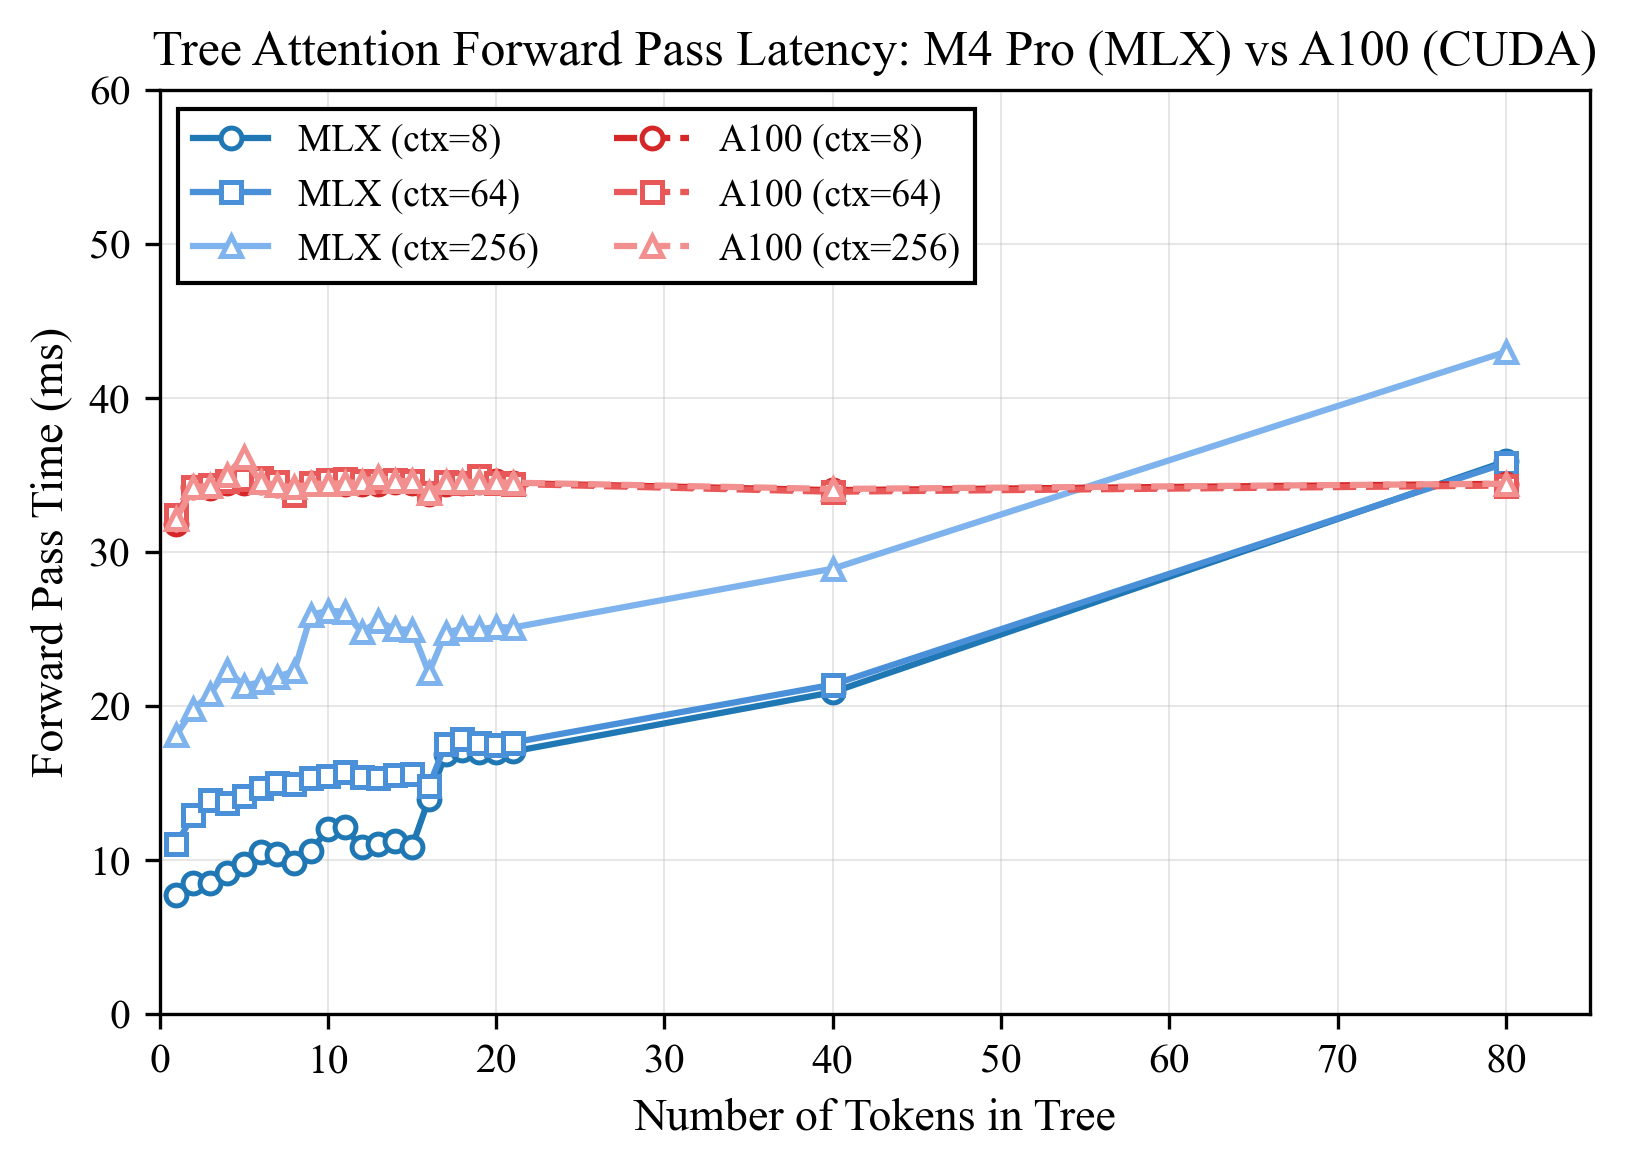
\includegraphics[width=0.6\linewidth]{figure2.png}
\caption{Profiling on MLX (M4 Pro) vs A100: tree size shifts backbone/verification cost.}
\label{fig:edge_profile}
\end{figure}

\begin{table}[t]
\caption{MLX results on GSM8K and HumanEval. Tok/Step = average tokens accepted per decoding step. Lite MTP is fastest.}
\label{tab:mlx_results}
\centering
\begin{minipage}{0.48\textwidth}
\centering
\small
\textbf{GSM8K}
\vspace{0.2em}

\begin{tabular}{lccc}
\toprule
\textbf{Mode} & \textbf{Tok/s} & \textbf{Tok/Step} & \textbf{Speedup} \\
\midrule
Baseline & 218.4 & 1.00 & 1.00$\times$ \\
Lite MTP & \textbf{234.4} & 1.39 & \textbf{1.07$\times$} \\
Lite MTP-3tok & 217.8 & 1.41 & 1.00$\times$ \\
Lite MTP-Depth2 & 215.9 & 1.48 & 0.99$\times$ \\
\bottomrule
\end{tabular}
\label{tab:mlx_gsm8k}
\end{minipage}
\hfill
\begin{minipage}{0.48\textwidth}
\centering
\small
\textbf{HumanEval}
\vspace{0.2em}

\begin{tabular}{lccc}
\toprule
\textbf{Mode} & \textbf{Tok/s} & \textbf{Tok/Step} & \textbf{Speedup} \\
\midrule
Baseline & 162.1 & 1.00 & 1.00$\times$ \\
Lite MTP & \textbf{208.6} & 1.36 & \textbf{1.29$\times$} \\
Lite MTP-3tok & 201.1 & 1.35 & 1.24$\times$ \\
Lite MTP-Depth2 & 201.1 & 1.43 & 1.24$\times$ \\
\bottomrule
\end{tabular}
\label{tab:mlx_humaneval}
\end{minipage}
\end{table}

\subsection{Edge Failure}

We then port the same MTP setup to Apple Silicon using MLX, again measuring decoding throughput \citep{hannun2023mlx}. However, the configurations that excelled on GPU were dramatically slower on-edge, the tok/s were between 3--5$\times$ slower relative to the MLX baseline. Examining the profiling in depth reveals that as tree size grows, verification becomes dominated by backbone and LM-head compute, and the expanded tree attention makes the backbone pass disproportionately expensive. Concretely, increasing tree size to 80 raises backbone cost by 3.17$\times$ on M4 Pro, while it increases only 1.12$\times$ on A100 \citep{apple2024m4, nvidia2020a100}. In this regime, most time is spent in the backbone pass, so the extra verification compute overwhelms the throughput gains from drafting more candidates.

\begin{table}[H]
\caption{Profiling Comparison (Context = 16). Backbone cost scales 3.17$\times$ on MLX vs 1.12$\times$ on GPU as tree size grows from 1 to 80.}
\label{tab:profiling}
\centering
\small
\begin{tabular}{c|ccc|ccc}
\toprule
& \multicolumn{3}{c|}{\textbf{MLX (M4 Pro)}} & \multicolumn{3}{c}{\textbf{GPU (A100)}} \\
\textbf{Tree Size} & \textbf{Backbone} & \textbf{Verify} & \textbf{Tok/s} & \textbf{Backbone} & \textbf{Verify} & \textbf{Tok/s} \\
\midrule
1 & 3.32ms & 4.62ms & 316.1 & 31.66ms & 31.57ms & 18.5 \\
2 & 3.56ms & 5.11ms & 299.5 & 38.49ms & 35.67ms & 19.0 \\
4 & 3.66ms & 5.70ms & 279.2 & 35.30ms & 35.60ms & 18.8 \\
8 & 3.69ms & 5.74ms & 331.5 & 35.56ms & 35.29ms & 21.2 \\
16 & 7.66ms & 10.60ms & 250.2 & 35.56ms & 35.37ms & 21.4 \\
80 & 10.53ms & 16.29ms & 223.7 & 35.71ms & 36.13ms & 22.2 \\
\bottomrule
\end{tabular}
\end{table}

\subsection{Minimalist Speculation}

Given the edge failure mode, we use sweeps over tree size (and context) to find the compute-optimal regime on-device. In an idealized sweep, the best tree size for M4 Pro is around 4, but this does not fully capture practical overheads in MLX (e.g., cache behavior when re-arranging KV state and Python overhead for restructuring tree attention). Empirically, tree size 2 is the most robust, our results show that it improves throughput from 218.4 to 234.4 tps (+7.3\%) on GSM8K, while larger trees tend to degrade performance \citep{cobbe2021gsm8k}. On HumanEval, tree size 2 improves 162.1 to 208.6 tps (+28.6\%), with larger trees still positive but weaker (+24\%) \citep{chen2021humaneval}. Given the consistent advantage of minimal trees, we present Lite MTP: a hardware-aware recipe for on-device inference using single-token, single-head speculation, where we keep verification overhead small enough to realize net speedups on Apple M4 Pro \citep{apple2024m4}.

\section{Conclusion}

We demonstrate that Multi-Token Prediction strategies optimized for GPUs, achieving up to 1.52$\times$ speedup on GSM8K and 1.64$\times$ on HumanEval, fail catastrophically on edge devices, resulting in 3-5$\times$ slowdowns due to insufficient FLOPs-to-bandwidth ratios to hide deep verification tree overhead. Lite MTP, our hardware-aware solution using single-token single-head speculation with compact dense heads, restores speedups of 1.07$\times$ on GSM8K and 1.29$\times$ on HumanEval on Apple M4 Pro while adding only 0.3\% parameter overhead (820k parameters), compared to 63--189\% for standard Medusa heads. This minimal footprint preserves the memory efficiency that makes SLMs viable for on-device deployment. Our findings suggest that effective edge speculation requires minimizing verification overhead rather than maximizing theoretical token yield.

\newpage
\begingroup
\small
\bibliography{references}
\endgroup
\bibliographystyle{iclr2026_conference}

\appendix

\end{document}
